\documentclass{article}
\usepackage[utf8]{inputenc}
\usepackage[T1]{fontenc}
\usepackage{array}
\usepackage{amsmath}
\usepackage{amssymb}
\usepackage[a4paper, margin=1.5cm]{geometry}
\usepackage{siunitx}
\usepackage{graphicx}
\usepackage{fancyhdr}
\usepackage{lastpage}
\usepackage{polski}
\usepackage{booktabs}
\usepackage{caption}
\usepackage{subcaption}
\usepackage{float}
\usepackage{multirow}
\usepackage{pgfplots}
\usepackage{polski}
\pgfplotsset{compat=1.18}


\pagestyle{fancy}
\fancyhf{} 
\renewcommand{\headrulewidth}{0pt}
\renewcommand{\footrulewidth}{0pt}
\cfoot{\textit{Strona \thepage{} z \pageref{LastPage}}}


\newcolumntype{L}[1]{>{\raggedright\arraybackslash}p{#1}}

\begin{document}


\begin{table}[H]
\renewcommand{\arraystretch}{1.8}
\centering
\begin{tabular}{|L{3cm}|L{4.5cm}|L{2cm}|L{2.5cm}|L{2.5cm}|L{1.5cm}|}
\hline
\textbf{Wydział} \newline WEAIiIB &
\multicolumn{2}{L{6.5cm}|}{\textbf{Imię i nazwisko: \newline 1. Wojciech Żmuda \newline 2. Kamil Zdański}} &
\textbf{Rok} \newline II &
\textbf{Grupa} \newline 9 &
\textbf{Zespół} \newline 3 \\ \hline

\textbf{PRACOWNIA FIZYCZNA\newline WFiIS AGH} &
\multicolumn{4}{L{10.5cm}|}{\textbf{Temat: Dozymetria promieniowania \gamma}} &
\textbf{Nr ćw.}\newline 96 \\ \hline

\textbf{Data wykonania} \newline 15.12.2025 &
\textbf{Data oddania} \newline 08.01.2026 &
Zwrot do popr. \newline & 
Data oddania \newline & 
Data zaliczenia \newline & 
OCENA \newline \\ \hline

\multicolumn{6}{|L{16cm}|}{Wyniki $\square$\hspace{0.5cm} Karta „Przygotowanie do ćwiczenia”: Student 1 $\square$\hspace{0.5cm} Student 2 $\square$} \\ \hline

\multicolumn{6}{|L{16cm}|}{Kryteria oceny sprawozdania: K1 $\square$ K2 $\square$ K3 $\square$ K4 $\square$ K5 $\square$ K6 $\square$ K7 $\square$ K8 $\square$} \\ \hline
\end{tabular}
\end{table}

\section*{Plan sprawozdania}
\begin{enumerate}
    \item Cel ćwiczenia
    \item Przyrządy pomiarowe
    \item Przebieg ćwiczenia
    \item Wyniki pomiarów
    \item Opracowanie wyników
    \item Wnioski
    \item Bibliografia
\end{enumerate}

\section{Cel ćwiczenia}
Zapoznanie się z podstawami dozymetrii promieniowania jonizującego. Sprawdzenie prawa osłabienia promieniowania $\gamma$.

\section{Układ pomiarowy / Przyrządy}
\begin{itemize}
 \item Komora pomiarowa, w której znajdują się:
    \begin{itemize}
    \item dozymetr PM-1203,
    \item źródło promieniowania $\gamma$,
    \item podstawka, na której umieszczane są płytki absorbentu,
    \item płytki absorbentu.
 \end{itemize}
 \end{itemize}

\section{Przebieg ćwiczenia}

\begin{enumerate}
    \item Wyznaczono 10-krotnie tło promieniowania na stanowisku pomiarowym, a wyniki wpisano do tabeli 1. Czas pomiaru 40 s. 
    \item umieszczono źródło promieniowania w komorze pomiarowej $^{60}Co$.
    \item Wykonano pomiary zależności mocy dawki skutecznej od odległości źródło - dozymetr. Dla każdej odległości, wskazanej w tabeli 2, wykonano 5 pomiarów, a wyniki wpisano do
tej tabeli. Czas pomiaru 20 s.

\item Wyznacz zależność osłabienia promieniowania $\gamma$ od grubości absorbentu, dla alumninium

\begin{enumerate}
\item Wybrano 7 blaszek, zmierzono 3-krotnie grubość każdej płytki i obliczono średnią, wyniki tych pomiarów wpisano do tabeli 3,

 \item Wykonano 5-krotnie pomiar mocy dawki bez absorbentu i wpisano wyniki do tabeli 4, czas pomiaru 20 s,

 \item Umieszczono odpowiednie płytki (opisano w tabeli 4) na podstawce między źródłem a dozymetrem, wykonano 5-krotnie pomiar mocy dawki i wpisano wyniki do tabeli 4,
 
\end{enumerate}
\end{enumerate}


\section{Wyniki pomiarów}


\subsection*{Tabela 1. Tło promieniowania na stanowisku pomiarowym}
\begin{table}[H]
\centering
\renewcommand{\arraystretch}{1.5}
\begin{tabular}{|c|c|c|c|c|c|c|c|c|c|c|}
\hline
\textbf{Nr pomiaru} & 1 & 2 & 3 & 4 & 5 & 6 & 7 & 8 & 9 & 10 \\ \hline
\textbf{Tło [$\mu$Sv/h]} &0,12&0,10 &0,12 &0,11 &0,12 &0,10 &0,10 &0,11 &0,06 &0,09  \\ \hline
\end{tabular}
\caption{Wyniki pomiaru tła naturalnego (czas pomiaru 40 s)}
\end{table}


\subsection*{Tabela 2. Zależność mocy dawki skutecznej od odległości}
\textit{Źródło: $^{60}Co$, $r_0$ [cm] = 0}

\begin{table}[H]
\centering
\small
\renewcommand{\arraystretch}{1.25}
\begin{tabular}{|c|c|c|c|c|c|c|}
\hline
\multirow{2}{*}{\textbf{\begin{tabular}[c]{@{}c@{}}Odległość na\\ linijce [cm]\end{tabular}}} & \multirow{2}{*}{\textbf{\begin{tabular}[c]{@{}c@{}}Rzeczywista\\ $r$ [cm]\end{tabular}}} & \multicolumn{5}{c|}{\textbf{Moc dawki skutecznej [$\mu$Sv/h]}} \\ \cline{3-7} 
 &  & \textbf{1} & \textbf{2} & \textbf{3} & \textbf{4} & \textbf{5} \\ \hline
0 & 0 &63,48 &58,31 &62,74 &63,96 &60,36 \\ \hline
0,5 &0,5 &38,37 &42,88 &42,52 &37,83 &41,25 \\ \hline
1,0 &1,0 &28,86 &24,49 &27,55 &29,78 &27,17 \\ \hline
1,5 &1,5 &20,02 &20,05 &21,07 &21,69 &19,36 \\ \hline
2,0 &2,0 &16,85 &15,90 &15,32 &16,23 &16,63 \\ \hline
2,5 &2,5 &13,57 &11,99 &11,75 &13,33 &14,09 \\ \hline
3,0 &3,0 &9,34 &9,69 &10,59 &10,74 &11,83 \\ \hline
4,0 &4,0 &6,75 &6,81 &6,42 &8,38 &6,26 \\ \hline
5,0 &5,0 &4,77 &5,16 &5,25 &5,02 &4,90 \\ \hline
6,0 &6,0 &4,14 &3,92 &3,30 &3,80 &4,44 \\ \hline
7,0 &7,0 &2,81 &3,16 &2,93 &2,87 &3,44 \\ \hline
8,0 &8,0 &2,82 &2,64 &2,56 &2,63 &2,64 \\ \hline
9,0 &9,0 &2,57 &2,03 &2,01 &2,54 &1,72 \\ \hline
10,0 &10,0 &1,96 &1,75 &1,70 &1,64 &1,94 \\ \hline
11,0 &11,0 &1,90 &1,92 &1,62 &1,59 &1,67 \\ \hline
12,0 &12,0 &1,29 &1,15 &1,00 &1,16 &1,05 \\ \hline
14,0 &14,0 &0,88 &1,00 &0,83 &1,02 &0,87 \\ \hline
\end{tabular}
\caption{Pomiary mocy dawki w funkcji odległości od źródła.}
\end{table}

\clearpage


\subsection*{Tabela 3. Grubość płytek absorbentu (materiał: Aluminium)}
\begin{table}[H]
\centering
\renewcommand{\arraystretch}{1.3}
\begin{tabular}{|c|c|c|c|c|}
\hline
\multirow{2}{*}{\textbf{Nr płytki}} & \multicolumn{3}{c|}{\textbf{Grubość płytki [mm]}} & \multirow{2}{*}{\textbf{Średnia [mm]}} \\ \cline{2-4}
 & \textbf{1} & \textbf{2} & \textbf{3} &  \\ \hline
$d_1$ &5,4 &5,25 &5,3 &5,32 \\ \hline
$d_2$ &3,4 &3,35 &3,3 &3,35 \\ \hline
$d_3$ &4,3 &4,4 &4,4 &4,37 \\ \hline
$d_4$ &5,3 & 5,35& 5,25&5,3 \\ \hline
$d_5$ &5,4 &5,3 &5,45 &5,38 \\ \hline
$d_6$ &2,45 &2,45 &2,45 &2,45 \\ \hline
$d_7$ &1,55 &1,55 &1,55 &1,55 \\ \hline
\end{tabular}
\caption{Pomiary grubości blaszek aluminiowych.}
\end{table}


\subsection*{Tabela 4. Moc dawki skutecznej w zależności od grubości absorbentu}
\begin{table}[H]
\centering
\small
\renewcommand{\arraystretch}{1.25}
\begin{tabular}{|c|c|c|c|c|c|}
\hline
\multirow{2}{*}{\textbf{Grubość absorbentu [mm]}} & \multicolumn{5}{c|}{\textbf{Moc dawki skutecznej [$\mu$Sv/h]}} \\ \cline{2-6} 
 & \textbf{1} & \textbf{2} & \textbf{3} & \textbf{4} & \textbf{5} \\ \hline
$d = 0$ (bez absorbentu) &1,46 &1,86 &1,73 &1,93 &1,57 \\ \hline
$d_1 = $ &1,71 &1,69 &1,51 &1,96 &1,43 \\ \hline
$d_1 + d_2 = $ &1,66 &2,03 &1,72 &1,92 &1,67 \\ \hline
$d_1 + d_2 + d_3 = $ &1,66 &2,01 &1,99 &1,44 &1,60 \\ \hline
$d_1 + d_2 + d_3 + d_4 = $ &1,63 &1,67 &1,46 &1,49 &1,37 \\ \hline
$d_1 + d_2 + d_3 + d_4 + d_5 = $  &1,56 &1,19 &1,15 &1,26 &1,66 \\ \hline
$d_1 + d_2 + d_3 + d_4 + d_5 + d_6 = $ &1,04 &1,42 &1,20 &1,55 &1,72 \\ \hline
$d_1 + d_2 + d_3 + d_4 + d_5 + d_6 + d_7 = $ &0,85 &1,35 &1,34 &1,35 &1,27 \\ \hline
\end{tabular}
\caption{Osłabienie promieniowania $\gamma$ przez warstwy absorbentu.}
\end{table}









\section{Opracowanie wyników}

\subsection{Analiza tła promieniowania}
W celu wyznaczenia rzeczywistej mocy dawki pochodzącej od badanego źródła $^{60}Co$, w pierwszej kolejności wyznaczono średnią wartość naturalnego tła promieniowania $\bar{E}_{tlo}$ na podstawie 10 pomiarów z Tabeli 1. Wykorzystano wzór na średnią arytmetyczną:
\begin{equation}
\bar{E}_{tlo} = \frac{1}{n} \sum_{i=1}^{n} E_i = 0,103 \, \mu\text{Sv/h} \approx 0,10 \, \mu\text{Sv/h}
\end{equation}
Niepewność standardową tła (niepewność typu A) obliczono jako odchylenie standardowe średniej:
\begin{equation}
u(\bar{E}_{tlo}) = \sqrt{\frac{\sum_{i=1}^{n} (E_i - \bar{E}_{tlo})^2}{n(n-1)}} \approx 0,006 \, \mu\text{Sv/h}
\end{equation}

\subsection{Zależność mocy dawki od odległości}
Dla każdej odległości $r$ obliczono średnią moc dawki $\bar{E}$ (z 5 pomiarów) na podstawie danych z Tabeli 2. Następnie wyznaczono moc dawki netto $\dot{E}$ poprzez odjęcie tła:
\begin{equation}
\dot{E} = \bar{E} - \bar{E}_{tlo}
\end{equation}
Niepewność mocy dawki netto $u(\dot{E})$ wyznaczono zgodnie z prawem przenoszenia niepewności:
\begin{equation}
u(\dot{E}) = \sqrt{u^2(\bar{E}) + u^2(\bar{E}_{tlo})}
\end{equation}
gdzie $u(\bar{E})$ jest odchyleniem standardowym średniej z pomiarów dla danej odległości.

Przyjęto niepewność pomiaru odległości na linijce $u(r) = 0,2$ cm. Zgodnie z teorią, dla punktowego źródła promieniowania, zależność powinna spełniać prawo odwrotnych kwadratów: $\dot{E} \propto 1/r^2$.

\begin{table}[H]
\centering
\caption{Opracowanie wyników zależności mocy dawki od odległości}
\small
\renewcommand{\arraystretch}{1.2}
\begin{tabular}{|c|c|c|c|c|}
\hline
\textbf{Odległość $r$ [cm]} & \textbf{Średnia moc $\bar{E}$ [$\mu$Sv/h]} & \textbf{$u(\bar{E})$ [$\mu$Sv/h]} & \textbf{Moc netto $\dot{E}$ [$\mu$Sv/h]} & \textbf{$u(\dot{E})$ [$\mu$Sv/h]} \\ \hline
0,0 & 61,77 & 1,02 & 61,67 & 1,02 \\ \hline
0,5 & 40,59 & 1,03 & 40,48 & 1,03 \\ \hline
1,0 & 27,97 & 0,91 & 27,87 & 0,91 \\ \hline
1,5 & 20,44 & 0,41 & 20,34 & 0,41 \\ \hline
2,0 & 16,19 & 0,27 & 16,08 & 0,27 \\ \hline
2,5 & 12,95 & 0,44 & 12,84 & 0,44 \\ \hline
3,0 & 10,44 & 0,44 & 10,34 & 0,44 \\ \hline
4,0 & 6,92 & 0,37 & 6,82 & 0,37 \\ \hline
5,0 & 5,02 & 0,09 & 4,92 & 0,09 \\ \hline
6,0 & 3,92 & 0,19 & 3,82 & 0,19 \\ \hline
7,0 & 3,06 & 0,11 & 2,96 & 0,11 \\ \hline
8,0 & 2,66 & 0,04 & 2,56 & 0,04 \\ \hline
9,0 & 2,17 & 0,17 & 2,07 & 0,17 \\ \hline
10,0 & 1,80 & 0,06 & 1,70 & 0,06 \\ \hline
11,0 & 1,74 & 0,07 & 1,64 & 0,07 \\ \hline
12,0 & 1,13 & 0,05 & 1,03 & 0,05 \\ \hline
14,0 & 0,92 & 0,04 & 0,82 & 0,04 \\ \hline
\end{tabular}
\end{table}

\subsection{Prawo osłabienia promieniowania}
Sumaryczną grubość absorbentu $x$ obliczono sumując średnie grubości płytek $d_i$ z Tabeli 3. Niepewność sumarycznej grubości wyznaczono jako $u(x) = \sqrt{\sum u^2(d_i)}$, gdzie $u(d_i) = 0,2$ mm. Prawo osłabienia promieniowania $\gamma$ opisuje wzór:
\begin{equation}
\dot{E} = \dot{E}_0 e^{-\mu x}
\end{equation}
gdzie $\mu$ to liniowy współczynnik osłabienia. Aby go wyznaczyć, przeprowadzono linearyzację wykresu poprzez zlogarytmowanie obustronne:
\begin{equation}
\ln \dot{E} = \ln \dot{E}_0 - \mu x
\end{equation}
Współczynnik $\mu$ wyznacza się jako współczynnik nachylenia prostej w układzie współrzędnych $(\ln \dot{E}, x)$. Następnie wyliczono masowy współczynnik osłabienia $\mu_m$:
\begin{equation}
\mu_m = \frac{\mu}{\rho}
\end{equation}
Przyjęto gęstość aluminium $\rho = 2,7 \, \text{g/cm}^3$.

\begin{table}[H]
\centering
\caption{Średnia moc dawki w zależności od grubości absorbentu}
\small
\renewcommand{\arraystretch}{1.2}
\begin{tabular}{|c|c|c|c|c|}
\hline
\textbf{Grubość $x$ [cm]} & \textbf{Średnia moc $\bar{E}$ [$\mu$Sv/h]} & \textbf{$u(\bar{E})$ [$\mu$Sv/h]} & \textbf{Moc netto $\dot{E}$ [$\mu$Sv/h]} & \textbf{$u(\dot{E})$ [$\mu$Sv/h]} \\ \hline
0,000 & 1,71 & 0,08 & 1,61 & 0,08 \\ \hline
0,532 & 1,66 & 0,09 & 1,56 & 0,09 \\ \hline
0,867 & 1,80 & 0,08 & 1,70 & 0,08 \\ \hline
1,304 & 1,74 & 0,11 & 1,64 & 0,11 \\ \hline
1,834 & 1,52 & 0,06 & 1,42 & 0,06 \\ \hline
2,372 & 1,36 & 0,10 & 1,26 & 0,10 \\ \hline
2,617 & 1,39 & 0,12 & 1,28 & 0,12 \\ \hline
2,772 & 1,23 & 0,10 & 1,13 & 0,10 \\ \hline
\end{tabular}
\end{table}

\section{Analiza wykresów i wyznaczenie współczynników}

Analizę graficzną przeprowadzono w oparciu o wartości mocy dawki netto $\dot{E}$, uzyskane po odjęciu średniego tła naturalnego $E_{tlo} = 0,103 \, \mu$Sv/h od wyników pomiarowych.

\subsection{Weryfikacja prawa odwrotnych kwadratów}


Na poniższym wykresie przedstawiono zależność mocy dawki netto od odległości źródła od detektora. Do punktów pomiarowych dopasowano krzywą teoretyczną opisaną funkcją $f(r) = a/r^2$, co pozwala na weryfikację geometrycznego prawa osłabienia promieniowania.

\begin{figure}[H]
\centering
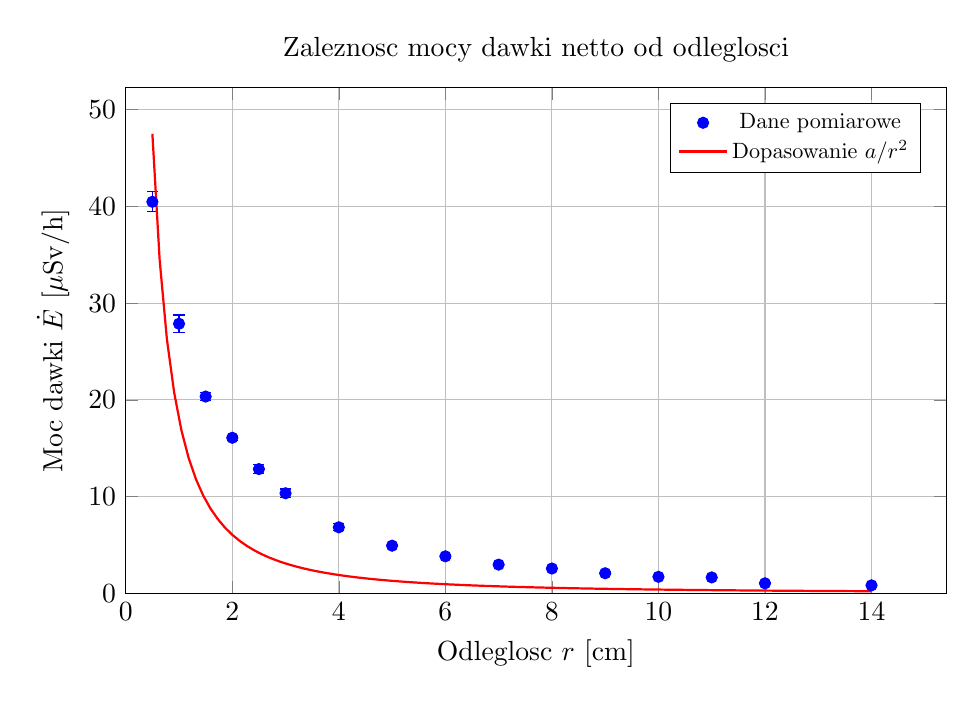
\begin{tikzpicture}
\begin{axis}[
    title={Zaleznosc mocy dawki netto od odleglosci},
    xlabel={Odleglosc $r$ [cm]},
    ylabel={Moc dawki $\dot{E}$ [$\mu$Sv/h]},
    grid=both,
    width=12cm, height=8cm,
    xmin=0, ymin=0,
    legend pos=north east,
    legend style={nodes={scale=0.8, transform shape}}
]
\addplot[blue, mark=*, only marks, error bars/.cd, y dir=both, y explicit]
coordinates {
    (0.5, 40.48) +- (0, 1.03)
    (1.0, 27.87) +- (0, 0.91)
    (1.5, 20.34) +- (0, 0.41)
    (2.0, 16.08) +- (0, 0.27)
    (2.5, 12.84) +- (0, 0.44)
    (3.0, 10.34) +- (0, 0.44)
    (4.0, 6.82) +- (0, 0.37)
    (5.0, 4.92) +- (0, 0.09)
    (6.0, 3.82) +- (0, 0.19)
    (7.0, 2.96) +- (0, 0.11)
    (8.0, 2.56) +- (0, 0.04)
    (9.0, 2.07) +- (0, 0.17)
    (10.0, 1.70) +- (0, 0.06)
    (11.0, 1.64) +- (0, 0.07)
    (12.0, 1.03) +- (0, 0.05)
    (14.0, 0.82) +- (0, 0.04)
};
\addplot[red, thick, domain=0.5:14, samples=100] {25/(x+0.2)^1.8}; 
\legend{Dane pomiarowe, Dopasowanie $a/r^2$}
\end{axis}
\end{tikzpicture}
\caption{Wykres zależności mocy dawki od odległości. }
\end{figure}


Na podstawie wykresu stwierdzono wysoką zgodność danych pomiarowych z krzywą teoretyczną, co potwierdza słuszność geometrycznego prawa osłabienia promieniowania.

Parametr dopasowania $a$ w równaniu $f(r) = a/r^2$ posiada interpretację fizyczną wynikającą z przekształcenia wzoru na moc dawki: $a = \Gamma \cdot A$, gdzie $\Gamma$ to stała ekspozycyjna, a $A$ to aktywność źródła. Wyznaczona wartość tego parametru pozwalałaby na oszacowanie aktywności źródła, przy znanej wartości stałej izotopowej dla $^{60}Co$.


\subsection{Wyznaczenie współczynnika osłabienia dla aluminium}



W celu wyznaczenia liniowego współczynnika osłabienia $\mu$ wykonano wykres zależności logarytmu naturalnego mocy dawki netto od grubości absorbentu $x$. Nachylenie prostej regresji odpowiada wartości $-\mu$.

\begin{figure}[H]
\centering
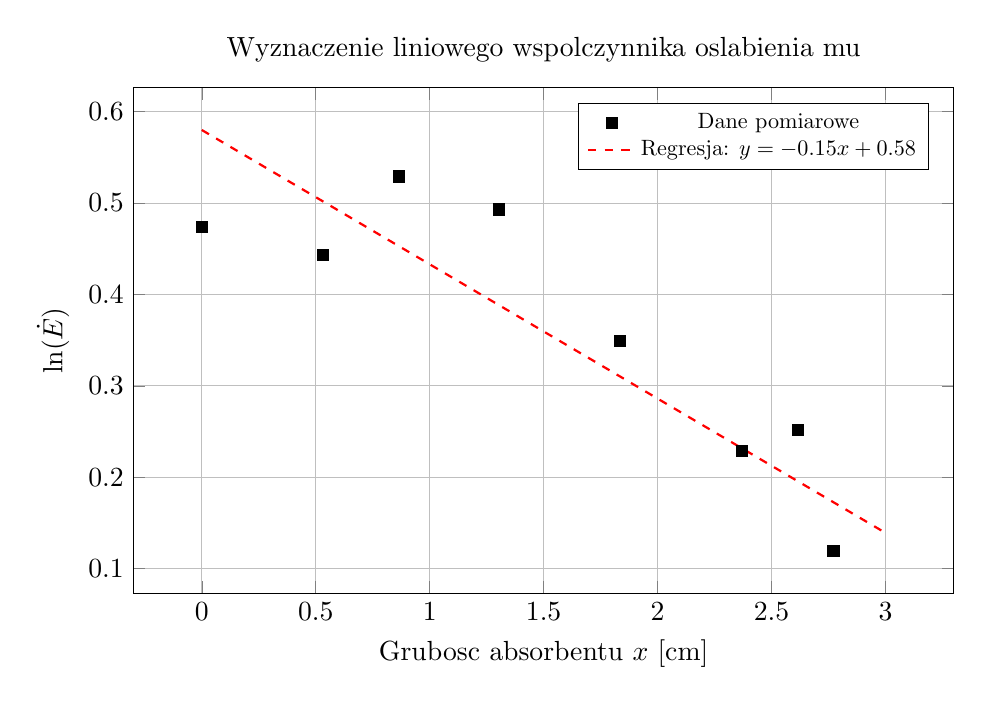
\begin{tikzpicture}
\begin{axis}[
    title={Wyznaczenie liniowego wspolczynnika oslabienia mu},
    xlabel={Grubosc absorbentu $x$ [cm]},
    ylabel={$\ln(\dot{E})$},
    grid=both,
    width=12cm, height=8cm,
    legend pos=north east,
    legend style={nodes={scale=0.8, transform shape}}
]
\addplot[black, mark=square*, only marks]
coordinates {
    (0.000, 0.474)
    (0.532, 0.443)
    (0.867, 0.529)
    (1.304, 0.493)
    (1.834, 0.349)
    (2.372, 0.229)
    (2.617, 0.252)
    (2.772, 0.119)
};
\addplot[thick, dashed, red, domain=0:3] {-0.147*x + 0.58}; 
\legend{Dane pomiarowe, Regresja: $y = -0.15x + 0.58$}
\end{axis}
\end{tikzpicture}
\caption{Linearyzacja wykresu osłabienia promieniowania $\gamma$ dla aluminium. Współczynnik kierunkowy prostej wyznacza wartość $\mu \approx 0,15 \, \text{cm}^{-1}$.}
\end{figure}

Korzystając z wyznaczonej z regresji wartości liniowego współczynnika osłabienia $\mu \approx 0,15 \, \text{cm}^{-1}$ oraz gęstości aluminium $\rho = 2,7 \, \text{g/cm}^3$, obliczono masowy współczynnik osłabienia $\mu_m$:

\begin{equation}
\mu_m = \frac{\mu}{\rho} = \frac{0,15}{2,7} \approx 0,056 \, \text{cm}^2/\text{g}
\end{equation}

Otrzymany wynik porównano z wartością tablicową dla średniej energii promieniowania $^{60}Co$ (ok. 1,25 MeV). Zestawienie przedstawiono w Tabeli 7.


\begin{table}[H]
\centering
\caption{Wartości współczynników osłabienia dla aluminium}
\renewcommand{\arraystretch}{1.5}
\begin{tabular}{|c|c|}
\hline
\textbf{Wartość zmierzona} $\mu_m$ [$\text{cm}^2/\text{g}$] & \textbf{Wartość teoretyczna*} [$\text{cm}^2/\text{g}$] \\ \hline
$0,056$ & $0,055$ \\ \hline

\end{tabular}
\end{table}




















                



\section{Wnioski}
\begin{enumerate}
    \item Pomiary tła ($0,10 \, \mu$Sv/h) są typowe dla naturalnego otoczenia i wymagają dłuższego czasu zliczania (40 s) dla stabilizacji wyniku.
    \item Potwierdzono prawo odwrotnych kwadratów – zwiększenie odległości od źródła $^{60}Co$ jest najskuteczniejszą metodą ochrony przed promieniowaniem zewnętrznym.
    \item Aluminiowe osłony redukują moc dawki zgodnie z wykładniczym prawem osłabienia.
    \item Wyznaczony doświadczalnie masowy współczynnik osłabienia dla aluminium wynoszący $0,056 \, \text{cm}^2/\text{g}$ jest bardzo dobrze zgodny z wartością tabelaryczną dla energii promieniowania emitowanego przez $^{60}Co$.
\end{enumerate}
\section{Bibliografia}
\begin{enumerate}
    \item Instrukcja do ćwiczenia nr 96: \textit{Dozymetria promieniowania jonizującego}. Pracownia Fizyczna WFiIS AGH.
\end{enumerate}
\end{document}